% Asset ID: AS2ForcesTikZ-005
% Source: Chapter 5/7 Forces Transcript + MechYr2 Chapter 5 Friction PDF
% Related lesson section: Core Theory: Inclined planes
% Purpose: Show mg sin(theta) down the slope and mg cos(theta) into the plane.
\documentclass[tikz,border=8pt]{standalone}
\usepackage{amsmath}
\usetikzlibrary{arrows.meta, angles, quotes, decorations.pathmorphing}
\begin{document}
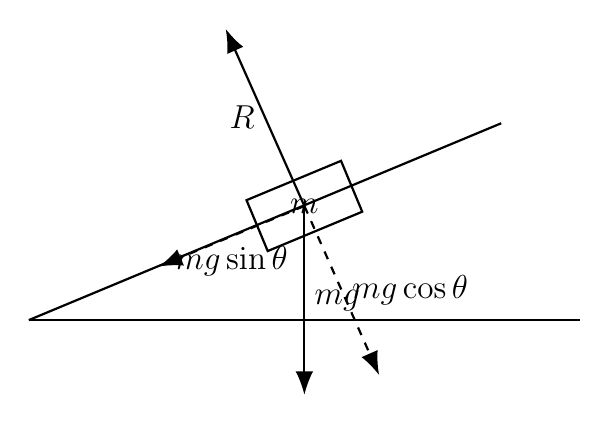
\begin{tikzpicture}[force/.style={-{Latex[length=3mm]}, thick}, comp/.style={-{Latex[length=3mm]}, thick, dashed}, label/.style={font=\large}, note/.style={font=\normalsize}]

\coordinate (A) at (0,0); \coordinate (B) at (7,0); \coordinate (C) at (6,2.5); \draw[thick] (A)--(B); \draw[thick] (A)--(C);
\begin{scope}[shift={(3.5,1.45)}, rotate=22.6]\draw[thick] (-0.65,-0.35) rectangle (0.65,0.35); \node[label] at (0,0) {$m$};\end{scope}
\coordinate (O) at (3.5,1.45); \draw[force] (O)--++(0,-2.4) node[midway,right,label] {$mg$};
\draw[force] (O)--++(-1.0,2.25) node[midway,left,label] {$R$};
\draw[comp] (O)--++(-1.85,-0.77) node[midway,below,label] {$mg\sin\theta$};
\draw[comp] (O)--++(0.95,-2.15) node[midway,right,label] {$mg\cos\theta$};
\end{tikzpicture}
\end{document}
